\chapter{Dimensionamiento de Subsistema de Navegación} \label{chp:dimensionamiento}

\vspace{0.2cm}


En este capítulo, se evalúa una opción de dimensionamiento de un subsistema de navegación que implica la estimación de componentes electrónicos necesarios, su capacidad y rendimiento requeridos para misiones near-space en HABs a partir de la perspectiva brindada del análisis exploratorio en función del tiempo de las diferentes variables estudiadas. Además, se tuvo en cuenta las restricciones técnicas y  COTS (comercial off-the-shelf) de los CubeSat  como filosofía desarrollo.

\vspace{0.7cm}

El dimensionamiento de subsistemas de navegación es un aspecto   <<ad hoc>> en este trabajo, que toma de referencias PyCubed, TASEC-Lab y propuesta abierta de comunidades de Hardware y Software.  Estas referencias provee los fundamentos de  las tecnologías de la misión estratosférica StratoBalloon con una experiencia que los respalda en aplicaciones similares.

\newpage

%%%%%%%%%%%%%%%%%%%%%%%%%%%%%%%%%%%%%%%%%%%%%%%%%%%%%%%%%%%%%%%%%%%%%%%%%%%%%%%%
%%%%%%%%%%%%%%%%%%%%%%%%%%%%%%%%%%%%%%%%%%%%%%%%%%%%%%%%%%%%%%%%%%%%%%%%%%%%%%%%

\section{Subsistema de Navegación}

La navegación en el marco de lo aeroespacial se refiere al conjunto de técnicas, procesos y sistemas utilizados para obtener la posición, velocidad y dirección de una aeronave durante su trayecto,  que se apoya de la observación aérea, terrestre y de los instrumentos de vuelo en función del tipo de aeronave el cual es altamente variado y depende de las características y requisitos específicos de cada plataforma \cite{understanding_gps, gnss}. Por ejemplo, en aeronaves convencionales (aviones comerciales, helicópteros, etc.)  se utilizan principalmente  sistemas como el sistema de navegación por satélites (GNSS, por sus siglas en inglés), sistema de navegación inercial (INS)  y radionavegación con los cuales se tiene una ubicación precisa y actualizada; no obstante, en nanosatelites compone de un sistema de nominado sistema de control de actitud (o en inglés, attitude control system abreviado ACS) con puesta por sensores y actuadores como magnetómetros, sensores de constelaciones, sensor solar \cite{attitude_componentes_nanosatelites}.  En el caso de los globos sonda, algunos elementos típicos de la navegación en aeronaves convencionales y nanosatélites pueden ser aplicables o estar ausentes debido a las características peculiares de esta plataforma.

Este dimensionamiento de subsistema de navegación se desarrolla para la misión experimental "StratoBalloon" que se consideró apropiado utilizar la filosofía CubeSat como fuente de referencia principal. Por lo anterior,  se aborda de manera \textit{ad hoc}, es decir, se desarrolla una propuesta solución buscando adaptarla y que sea funcional como primera aproximación  para obtener  información relativa del seguimiento de la trayectoria del globo sonda, así como para recopilar el dato meteorológico de temperatura. Por lo tanto, en el caso particular de StatoBalloon,  los elementos que se retoman y su utilidad en el subsistema de navegación para el globo sonda son:

\begin{enumerate}
    \item \textbf{GNSS:} determina la ubicación del globo-sonda mediante las diferentes señales de las constelaciones satelitales existentes.
    \item \textbf{Sensor inercial:} también conocidos como Inertial measuremten unit (IMU), estos sensores miden la aceleración y la velocidad angular para obtener información sobre los movimientos y cambios de dirección.
    \item \textbf{Sensor barométrico:} mide la altitud en función de la variación de la presión atmosférica. 
\end{enumerate}

\textbf{Adicionales}: un microcontrolador dedicado para el subsistema como On board computer (OBC), memoria de datos y  un sensor de temperatura. Estos elementos adicionales podrían no tener sentido en la navegación propia o podrían ser  suprimidos. Se ha obviado el hecho de tener alimentación y gestión energética en el subsistema de navegación, además de un sistema de telecomunicaciones o telemetría, y también a cualquier otro subsistema que adicione StratoBalloon.

\newpage

\section{Criterios de Selección}

Existieron dos criterios de selección de componentes electrónicos: generales y simulación. Los criterios generales se basan en una forma de como diseñar un dimensionamiento tomando como principios un rápido y amigable desarrollo de estas tecnologías; por otro lado, los criterios de simulación se toman los datos de las variables que puede llegarse a medir a lo largo de la trayectoria para estimar que necesidad se tiene de equipo a utilizar.  A continuación se detallan los criterios:

\subsection{Generales}

\begin{itemize}

    \item Uso de componentes comerciales, usando el modelo COTS (comercial off-the-shelf) típico en nanosatélites.  Esto favorece la adquisición de repuestos y la compatibilidad con otros sistemas en el futuro.
    \item Obtener componentes electrónicos, considerando cuidadosamente  la calidad, el precio, precisión ofrecidos en el mercado.

    \item Buen soporte y documentación de las tecnologías o herramientas. De esta forma, se busca que los tiempos de desarrollo sean cortos, seleccionando tecnologías que nos permita alcanzar mejores resultados de manera eficiente.
    \item Optar por una modularidad e interoperabilidad entre los componentes, así permite una mayor flexibilidad, compatibilidad e integración con respecto a la configuración y actualización de los equipos.
\end{itemize}

\subsection{Simulación}

\begin{itemize}
    \item Poseer la mejor resistencia a las condiciones ambientales adversas de la atmósfera, como podrían ser robustez a cambios de temperatura y si es posible a la humedad, a pesar de no estar considerada en la simulación. En figura \ref{fig:atmosferica_altitud} y figura \ref{fig:atmosferica_tiempo} se mostró estas condiciones  adveras, exceptuando humedad. Además, se debe de considerar el tiempo de duración de la misión, que según la simulación del capítulo \ref{chp:02_simulacion}  de 2.5 horas.
    \item Cuidar el tamaño y peso de los elementos debido a que afecta en las ecuaciones \ref{eq:ascenso} y \ref{eq:descenso} relativo a la dinámica del sistema. Además, ayuda a que en un futuro poder optimizar el espacio y minimizar el peso total del sistema.
    \item Buscar la mejor eficiencia energética  en términos de consumo debido a que el recurso energético es limitado e influenciado por las condiciones adversas del ambiente \cite{condiciones_entorno_baterias}. 

\end{itemize}

\section{Componentes del Subsistema de Navegación}
 
Los componentes analizados se seleccionaron entre aquellos disponibles en el mercado local del país, buscando aquellos que ofrezcan las mejores prestaciones posibles, luego de ello,  se analizó la disponibilidad con diferentes vendedores, tiendas  y distribuidores internacionales de componentes electrónicos investigados\footnote{Se deja de lado las empresas de manufactura debido a comúnmente subcontratan la venda de sus productos y además no vende al por menor.} se mencionan algunos de ellos: como mayorista Mouser Electronics y Digi-key; como distribuidores minoristas y compañías de hardware de código abierto como Sparkfun y Adafruit. Además, se retomó componentes de algunas investigaciones  probados en condiciones similares a las mostradas por el simulador desarrollado en este trabajo.  En anexo \ref{chp:anexo:componentes_analizados&extras} se colocan diferentes componentes analizados en este trabajo, a continuación se detalla cada componente seleccionado para el subsistema:

\begin{itemize}
    \item \textbf{NEO-M9N GPS Breakout:}  es una placa desarrollada por SparkFun siendo un módulo receptor GNSS de 92 canales que puede recibir señales de los sistemas Galileo, GPS, GLONASS,  y BeiDou lo que mejora la precisión (apróx. 1.5 metros) y reduce el tiempo de sintonización,  cuenta con un conector tipo SMA para colocar la antena de preferencia. Además, es altamente configurable con el software u-center de la compañía Suiza u-blox \footnote{Software del fabricante: \url{https://www.u-blox.com/en/product/u-center}}.  Este es el único elemento que no está presente en algún estudio, se seleccionó por su alta prestaciones y precisión al tener alta disponibilidad de constelaciones satelitales;  los datos de posición de latitud, longitud analizados en el simulador aparentemente puede tener la presión según modelos matemáticos usados y la forma de resolver los modelos, viendo la importancia de obtener los mejores datos de posición (alta disponibilidad y la mejor presión) se seleccionó este equipo, además de su alta documentación y respaldo de SparkFun. En figura \ref{fig:gnss} se muestra el módulo.

    \begin{figure} [h]
        \centering
        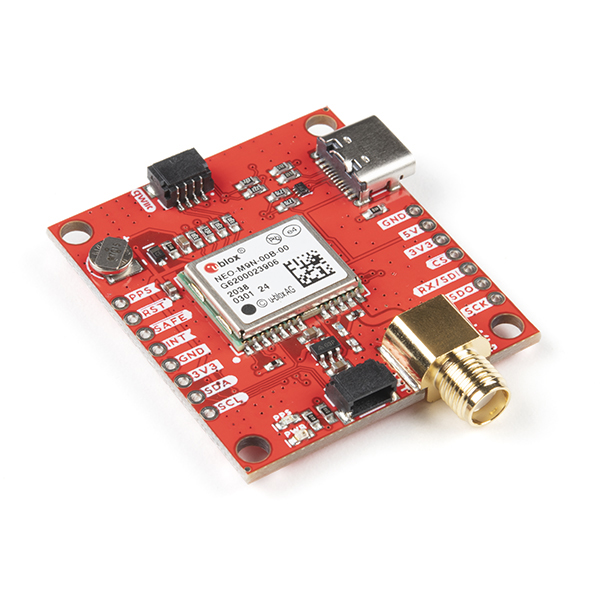
\includegraphics[width=0.25\linewidth]{document/figures/04_GPS__NEO-M9N__SMA__qwiic_sparkFun.jpg}
        \caption{GPS Breakout, Créditos a SparkFun CC BY 2.0, sin edición.}
        \label{fig:gnss}
    \end{figure}

    \item \textbf{Registro de vuelo:}  se utiliza OpenLog de Sparkfun y una tarjeta microSD SanDisk High Endurance, con los cuales se almacena y registra datos durante el vuelo,  esto permite capturar y analizar datos meteorológicos y variables del globo sonda para su posterior estudio para fines científicos o de depuración. El criterio de selección de la microSD fue dada por  \cite{sd_pycubed, pycubed}. En figura \ref{fig:openlog} y figura \ref{fig:microsd}  se muestran los dispositivos/
\begin{figure}[h]
    \centering
    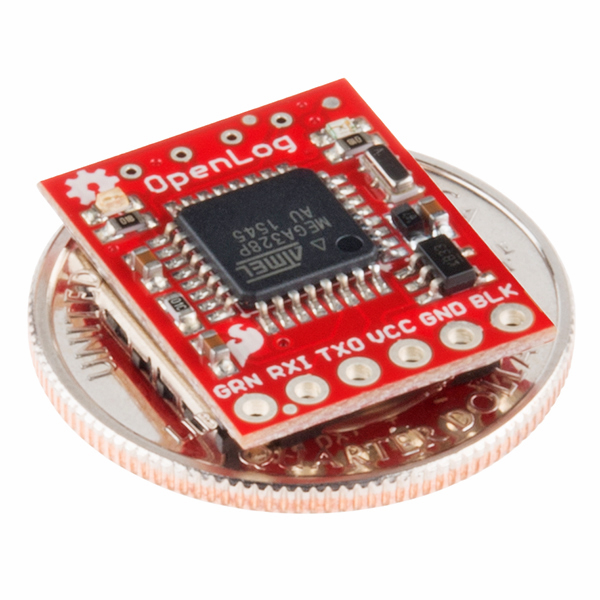
\includegraphics[width=0.25\linewidth]{document/figures/04_OpenLog_SparkFun.jpg}
    \caption{OpenLog. Créditos a SparkFun CC BY 2.0, sin imagen edición}
    \label{fig:openlog}
\end{figure}

\begin{figure}[h]
    \centering
    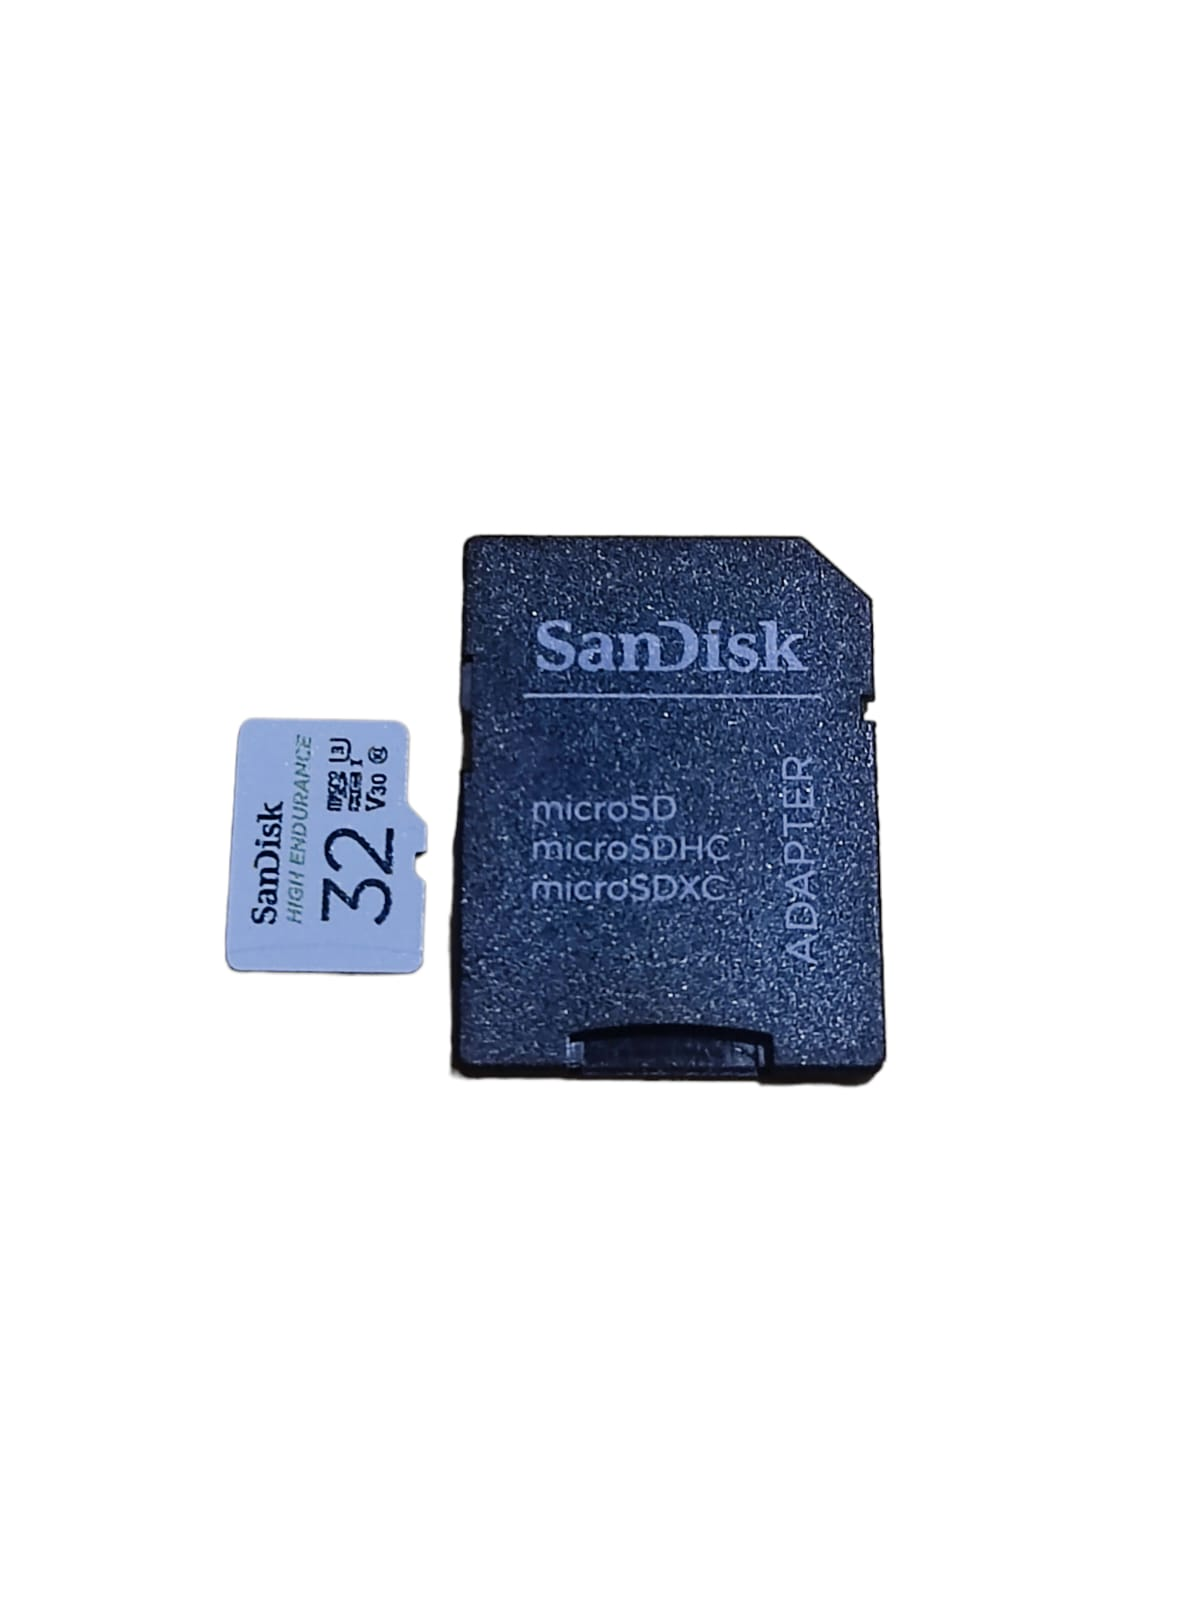
\includegraphics[width=0.35\linewidth]{document/figures/04_microSD_propia.jpg}
    \caption{MicroSD Sandisk High Endurance.  Fotografía, autoría propia}
    \label{fig:microsd}
\end{figure}

    \item \textbf{MS5611-01BA03}:  es un sensor de presión barométrica de alta precisión con un rango de operación de 10 a 1200 hPa acorde con gráfica de figura \ref{fig:atmosferica_tiempo} y \ref{fig:atmosferica_altitud},  ampliamente utilizado en aplicaciones que requieren mediciones exactas de altitud y control de altitud en dispositivos como drones, aviones y estaciones meteorológicas. Este sensor fue utilizado en estos trabajos \cite{pycubed, TASEC_Lab, navio_componentes}. En figura \ref{fig:MS5611} se muestra el dispositivo.

\begin{figure}[h]
    \centering
    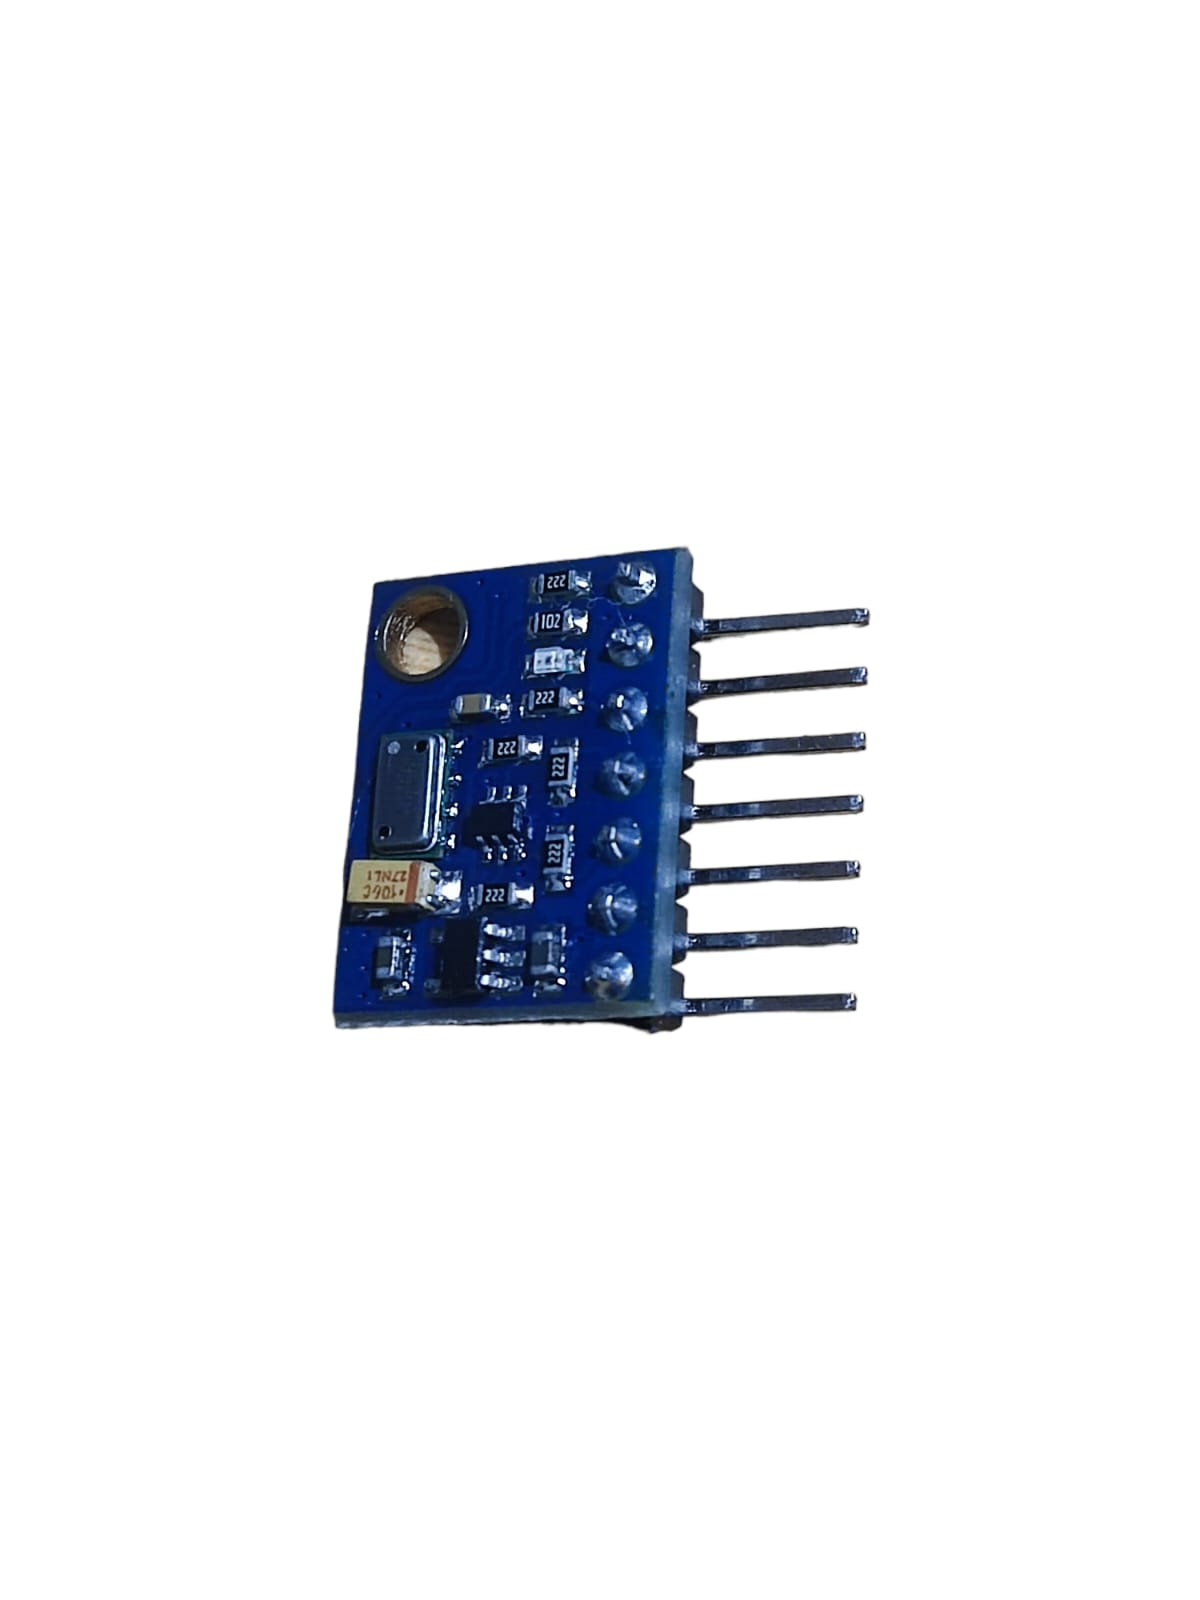
\includegraphics[width=0.25\linewidth]{document/figures/04_MS5611-01BA03_propia.jpg}
    \caption{Módulo genérico MS5611-01BA03.  Fotografía, autoría propia}
    \label{fig:MS5611}
\end{figure}

    \item \textbf{LSM9DS1:} la  se utiliza como IMU (inertial measurement unit) obedece a tener información del movimiento con su dirección y orientación del globo sonda, este IMU cuenta con 9 grados de libertad contando con un acelerómetro, magnetómetro y giroscópico de tres ejes todos respectivamente. Este sensor fue utilizado en estos trabajos \cite{pycubed, TASEC_Lab, navio_componentes}, además es ampliamente utilizado como complemento de GNSS para aumentar su precisión \cite{gnss}. En figura \ref{fig:imu} se muestra el equipo.

\begin{figure} [h]
    \centering
    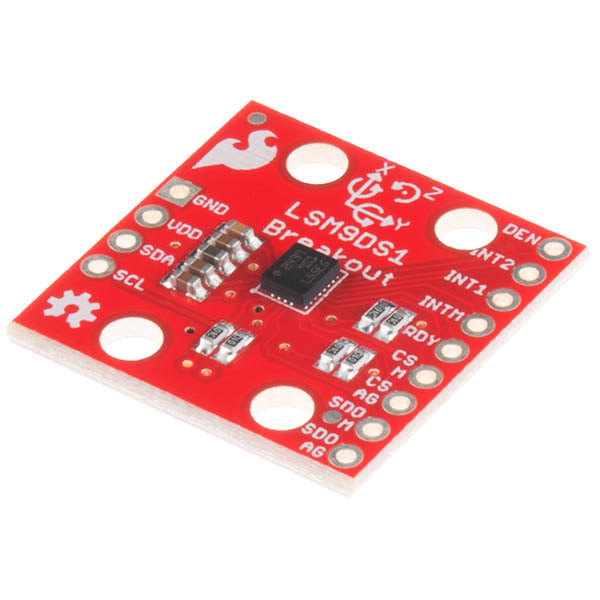
\includegraphics[width=0.25\linewidth]{document/figures/04_LSM9DS1_sparkfun.jpg}
    \caption{LSM9DS1, Créditos a SparkFun CC BY 2.0,  sin edición}
    \label{fig:imu}
\end{figure}

    \item \textbf{PT1000:}   los detectores de temperatura de resistencia (RTD) son sensores de temperatura que contienen una resistencia que cambia el valor de resistencia a medida que cambia su temperatura, la resistencia es en realidad una pequeña tira de platino con una resistencia de 1000 ohmios a 0 °C, de ahí el nombre PT1000. En comparación con la mayoría de los termistores NTC/PTC, el tipo PT de RTD es mucho más estable y preciso. En TASEC-Lab fueron utilizados para la caracterización dinámica del vuelo, así como también para conocer la convección de la atmosfera durante su experimento \cite{TASEC_Lab}. Se le adicionó un amplificador llamado MAX3186 desarrollado por Adafruit con el objetivo de facilitar el desarrollo, en figura \ref{fig:pt100+max} se aprecian ambos elementos. 

\begin{figure}[h]
    \centering
    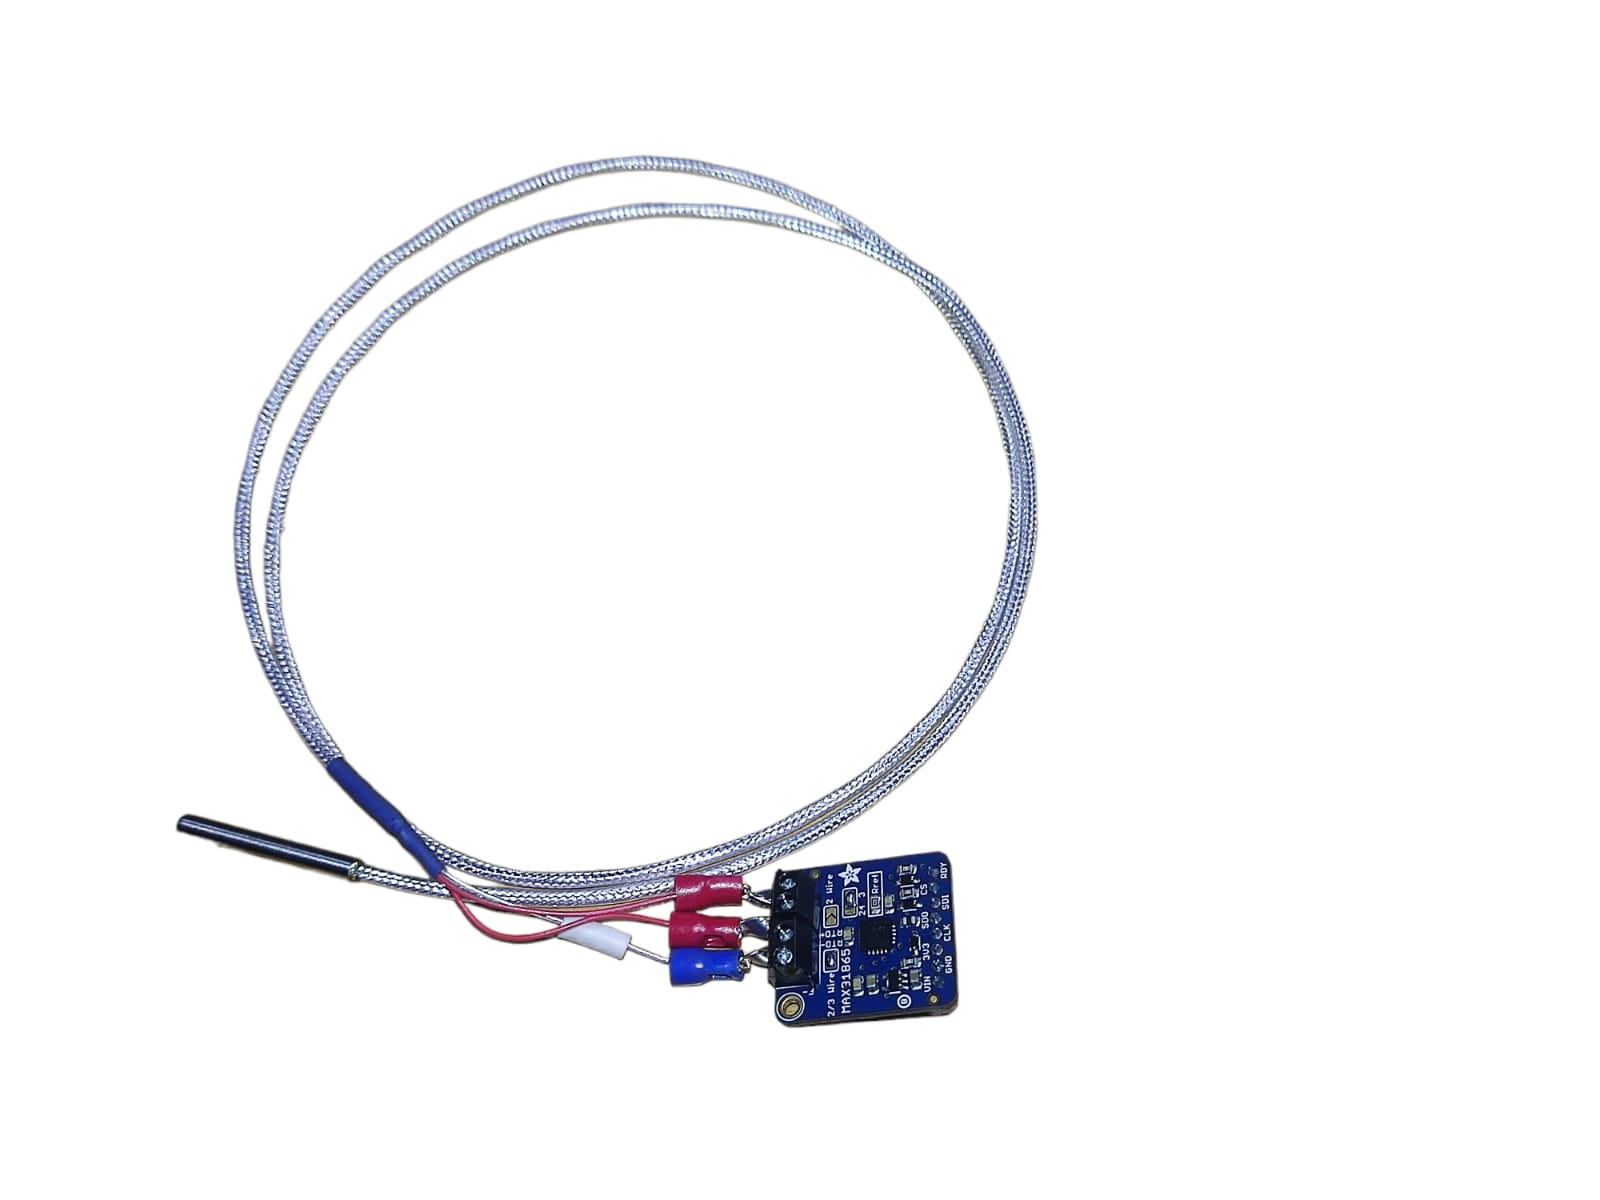
\includegraphics[width=0.5\linewidth]{document/figures/04_PT1000+MAX_propia.jpg}
   \caption{PT1000 junto con MAX31865 RTD. Fotografía, autoría propia}
    \label{fig:pt100+max}
\end{figure}

\item \textbf{Computadora a abordo:}  Es la unidad de procesamiento, responsable de recibir y procesar los datos E/S  provenientes de los diferentes  componentes con anterioridad mencionados. Se plateó utilizar  Arduino Nano V3 o SMT32 NUCLEO-L432KC debido se pueden intercambiar porque poseen el mismo socket (conector), las hojas técnicas mostró  que el STM32 posee características de duplicar en casi todo al Arduino, además posee un IDE con mejor integridad y mayor configurabilidad y más avanzado.   En figura \ref{fig:micro}, se muestra un Arduino Nano de forma ilustrativa para mostrar el socket.

\begin{figure}[h]
    \centering
    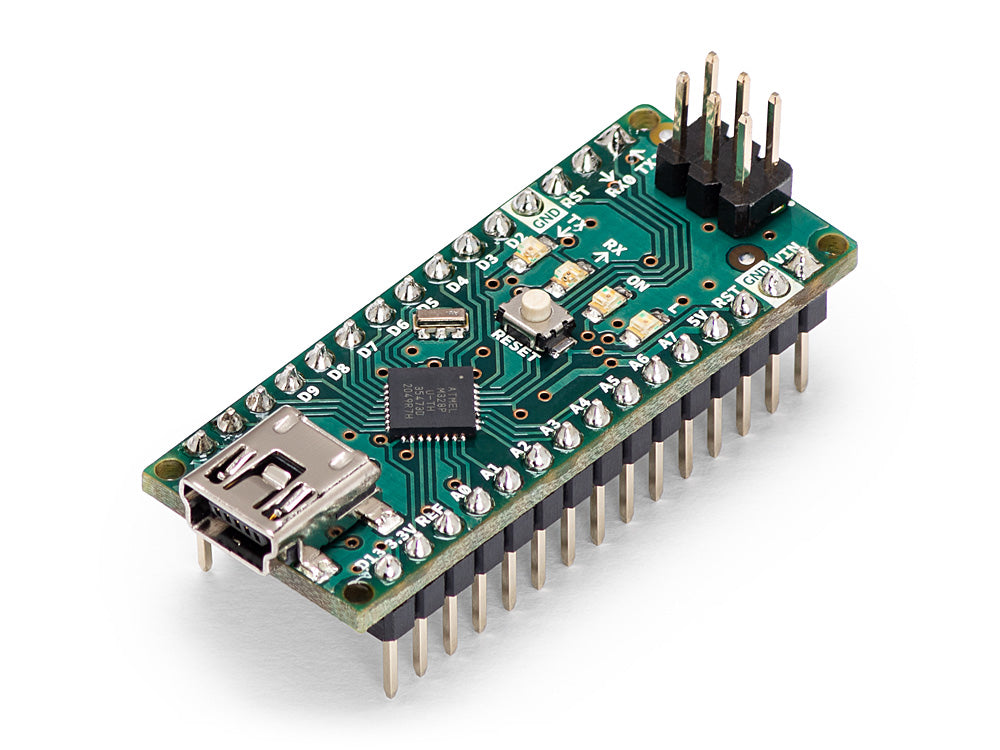
\includegraphics[width=0.25\linewidth]{document/figures/04_arduino_nano_v3.jpg}
    \caption{Arduino Nano Rev3.  Créditos a Arduino CC, CC BY-SA 4.0}
    \label{fig:micro}
\end{figure}

\end{itemize}

\vspace{0.5cm}

Todos los elementos mostrados son adecuados para la operación del globo sonda en las condiciones de temperatura y presión simuladas. Se seleccionaron componentes con alta documentación y pruebas en misiones similares y ninguno de los elementos mencionados es inflexible a cambios,  se buscó aproximar el mejor dimensionamiento. Se recomienda revisar los anexos para obtener información detallada sobre peso, consumo energético, dimensiones 3D y documentación específica de cada componente.

\newpage

\section{Dimensionamiento de Subsistema de Navegación}

Las dimensiones físicas de la PCB (Printed Circuit Board) se decide que son 12x8 cm y los componentes no mayores de 2.4 cm de altura, ya que esta es la división de los niveles entre cada subsistema, retomándose del trabajo anterior desarrollado en le marco StratoBalloon \cite{tesis_estructura_stratoballoon}. En el presente subsistema de navegación, por la selección realizada en los componentes, se  tienen conjunto de \textit{"módulos de placas de circuitos"} montados sobre una placa madre, siendo así que el diseño de los circuitos se ha aprovechado de la técnica de prototipado rápido y modular, lo cual permite agilizar el proceso de desarrollo.

\begin{figure}[h]
    \centering
    \includegraphics[width=0.95\linewidth]{document/figures/04_ckto_navegación.png}
    \caption{Diagrama de bloques del dimensionamiento.}
    \label{fig:diagrama_dimensionamiento}
\end{figure}

En la figura \ref{fig:diagrama_dimensionamiento} se presentan las conexiones. En el subsistema de navegación, se intentó que todos componentes internos tuvieran una conexión I2C  por la alta versatilidad que estos ofrecen, ejemplo de ello es el sistema de conexión Qwicc desarrollado por SparkFun \cite{qwiic}.  El registro de vuelo y sensor de temperatura debido a que solamente los protocolos UART y SPI  poseían respectivamente fueron los únicos con los que no se trabajó con I2C Por otro lado, los demás subsistemas (telemetría y energía) se proyecta que tengan una comunicación entre sus computadoras abordo con el protocolo I2C, sin embargo, en el marco StratoBalloon estos detalles pueden cambiar según necesidades de diseño y planeación.

\newpage

En este dimensionamiento, se ha omitido abordar aspectos más específicos relacionados con los subsistemas como telemetría y energía y solamente se consideró su comunicación y alimentación recibida por ellos,  sin embargo,  recuérdese que se trata de un proyecto que debe articularse con las diferentes partes involucradas (ver figura \ref{fig:diagrama_dimensionamiento}) y es necesario desarrollar pruebas de funcionamiento del mismo tanto en condiciones de simulación como en funcionalidad de software y hardware;  dejándose aquí establecido lo más adecuado con las características necesarias para asegurar el funcionamiento más óptimo posible de un subsistema de navegación y teniendo en cuenta los requisitos y las limitaciones de la misión con la simulación de trayectoria. Dicho lo anterior, se procede mostrar la disposición de los conjuntos de \textit{"módulos de placas de circuitos"} montados sobre una placa madre, como se muestra en figura \ref{fig:layout}, diseño de placa desarrollado en Fusion360.

\begin{figure} [h]
    \centering
    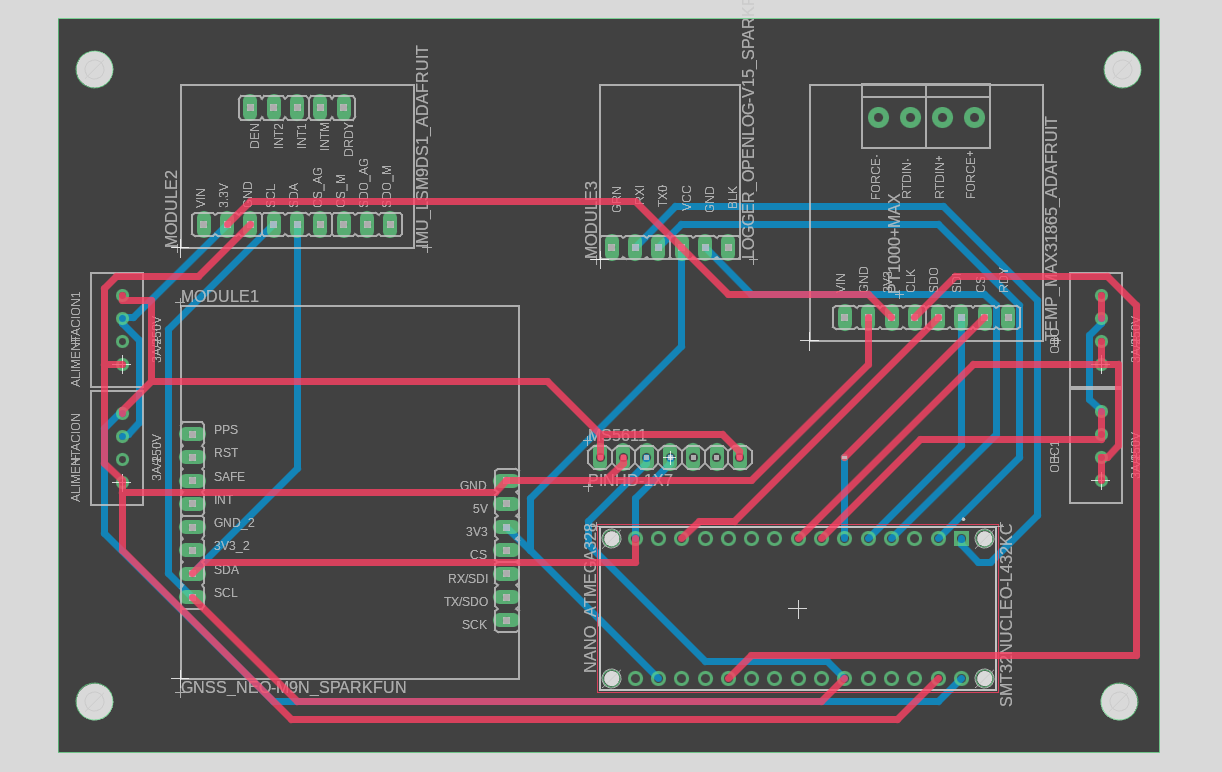
\includegraphics[width=0.75\linewidth]{document/figures/04_layout.png}
    \caption{Disposición de las pistas de la PCB, layout. }
    \label{fig:layout}
\end{figure}

El diseño es muy preliminar y puede estar sujetos a cambios, sin embargo, se tomaron ciertas consideraciones al momento de diseñar lo mostrado en figura \ref{fig:layout}:
\begin{itemize}
    \item Los laterales cortos (8 cm) de la placa son utilizados para la alimentación de energía y comunicación  con las diferentes placas que se proyectaron \cite{tesis_estructura_stratoballoon}.
    \item Todos los agujeros en los bordes de la placa tienen una dimensión de 4 mm de diámetro, útiles para facilitar el montaje y la fijación en la posible estructura de referencia \cite{tesis_estructura_stratoballoon}; y con respecto a la ubicación de cada agujero, están a una distancia de 5.5 mm con respecto al lateral de 8 cm y 4 mm con respecto al lateral de 12 cm, véase figura \ref{fig:agujeros_placa} amplía más esta idea y se puede consultar demás detalles en anexos \ref{chp:anexo:source_thesis}.

    \item Los conectores usados tanto para alimentación como para comunicación son JST B4B-XH-A, se usan por su alta versatilidad y disponibilidad en el mercado.
\end{itemize}

Con las anteriores consideraciones listadas, no se tomaron más consideraciones ni se siguieron estándares debido a lo complejo que pueden llegar hacer para una industria aeroespacial tan exigente, como también que este dimensionamiento es una tecnología introductoria que se espera que seguía desarrollando en el marco de StratoBalloon. Ejemplos de estándar podría ser PC104\footnote{Más información en la página oficia, es un estándar muy usual en nanosatélites. Link: \url{https://pc104.org/pc104-consortium/}} o consideraciones como distribución del calor o convección de los subsistemas a partir de simulaciones más complejas.  

\begin{figure}[h]
    \centering
    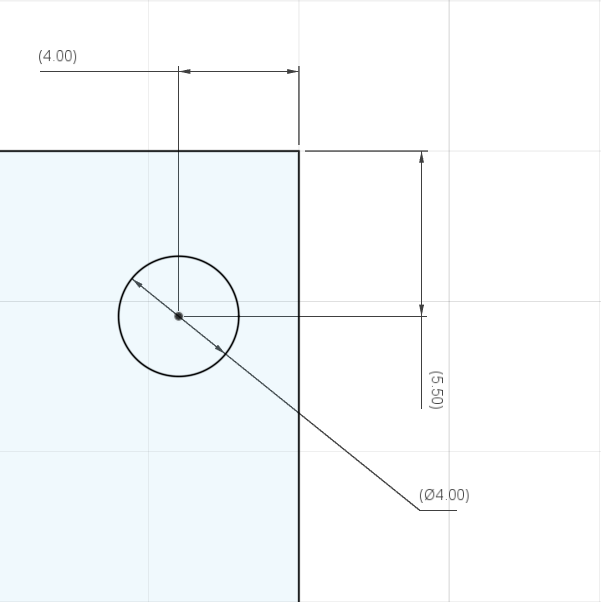
\includegraphics[width=0.75\linewidth]{document/figures/04_disposicion_agujero_PCB.png}
    \caption{Disposición de los agujeros en placa}
    \label{fig:agujeros_placa}
\end{figure}
\newpage
\begin{figure}[h]
    \centering
    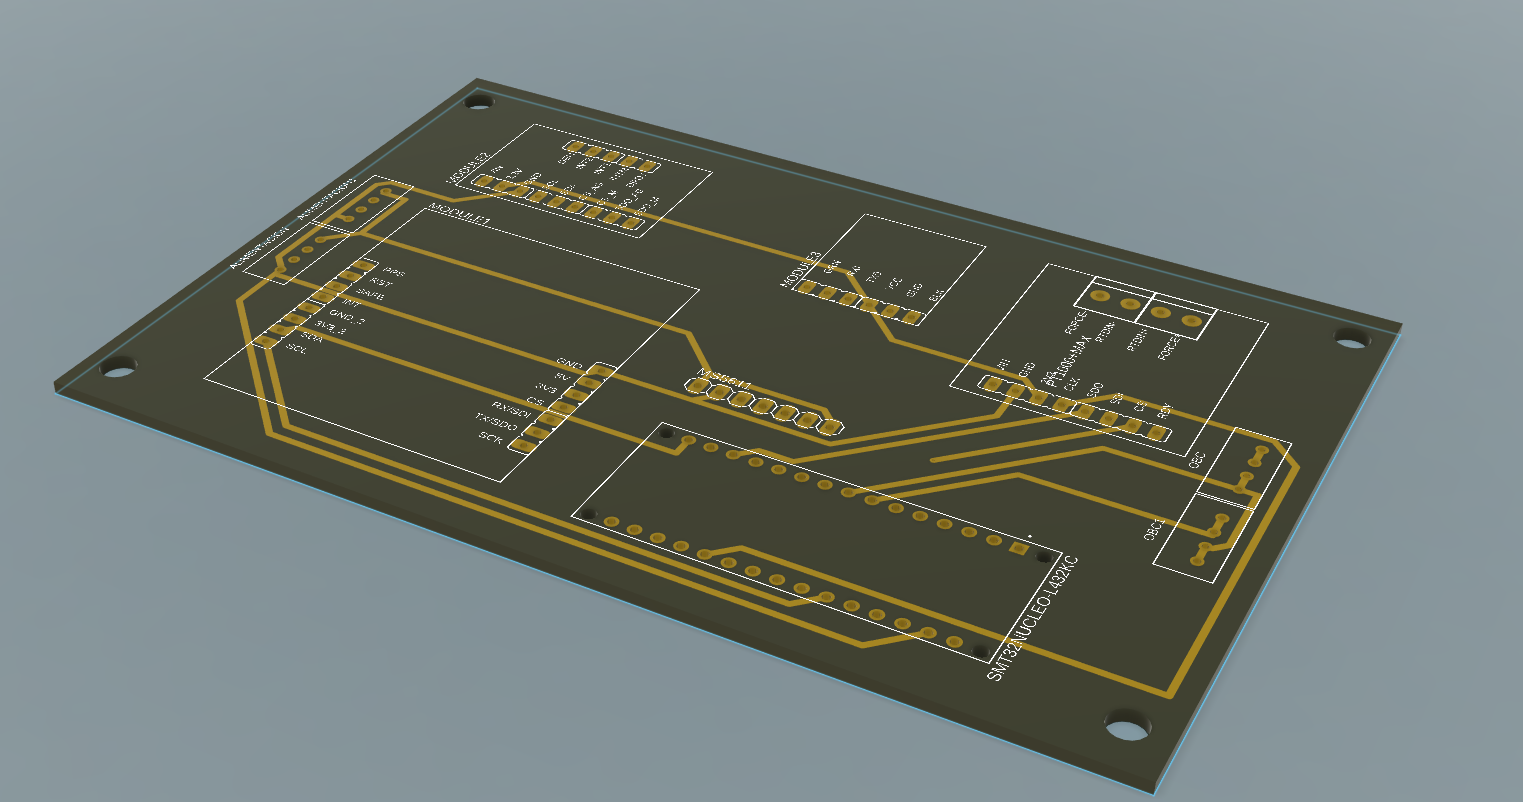
\includegraphics[width=1\linewidth]{document/figures/04_PCB v1_3D.png}
    \caption{Placa de Circuito en 3D.}
    \label{fig:PCB_3D}
\end{figure}

La figura \ref{fig:PCB_3D} muestra una representación en tres dimensiones de una placa que está lista para ser utilizada en prototipos y pruebas. El propósito de estas pruebas es evaluar la funcionalidad de cada componente dentro del contexto de la misión. La estrategia utilizada se basa en la idea de crear \textit{"módulos de placas de circuitos"} que serán ensamblados en una placa madre. Esta estrategia de diseño y ensamblaje se puede implementar en los laboratorios de la Universidad Don Bosco. Aunque en la fabricación actual no se usaron los archivos Gerber, estamos considerando generarlos para un posible proceso de manufactura futuro. Esto implica que el diseño actual podría ser adaptado y optimizado en una sola placa en caso de que se decida avanzar en la producción a lo largo de StratoBalloon. 

La manufactura en el extranjero, asumiéndose una optimización del diseño anterior de figura \ref{fig:PCB_3D},  se tiene que en cuanto a los parámetros de fabricación, se debe tener en cuenta el fabricante seleccionado y el tipo de material utilizado en la manufactura son factores determinantes. Se sugiere utilizar FR4 estándar para prototipos y FR408HR para la versión final de vuelo en futuras misiones; para el diseño con FR408HR, se especifica una impedancia controlada de 50 ohmios, con anchos de traza externos de 11 mils y anchos de traza internos de 10.7 mils según \cite{pycubed}.

\newpage

Es relevante destacar que la elección de los componentes electrónicos se llevó a cabo con base en hojas técnicas y datos ambientales adquiridos a través de simulaciones en capítulo \ref{chp:03_eda}. A pesar de que estos datos no replican directamente las condiciones reales de una misión, proporcionan una aproximación significativa que disminuye el riesgo al obtener información durante un vuelo en gloo estratosférico. Los detalles completos y respaldos de esta selección se encuentran en el anexo \ref{chp:anexo:componentes_analizados&extras}. En dicho anexo, se presentan tablas que muestran la temperatura de operación, la sensibilidad, el peso, el consumo y otros parámetros relevantes de los componentes. 

En anexo \ref{chp:anexo:pcb_layout_esquematico} se puede observar el diagrama esquemático y layout. Además, los archivos generados en este capítulo se pueden consultar con las indicaciones dadas en anexo \ref{chp:anexo:source_thesis}

